\documentclass[a4paper]{article}

\usepackage[utf8]{inputenc}	% Flere sprog tegnsæt (fx æøå)
\usepackage[english]{babel}	% Dansk orddeling (kan ændres til english)
\usepackage[T1]{fontenc}		% Brug 8-bit front
\usepackage{lmodern}		% Vektor front

\usepackage[svgnames]{xcolor} % Udvider \color med "SVG color names"
\usepackage{graphicx}	% Kompatibilitet til visning af pixel billeder (.png, .jpg, .gif)
\usepackage{epstopdf}	% Kompatibilitet til visning af vector billeder (.eps)
\usepackage{parskip}	% Tilføjer vertikal margin til hver paragraph
\usepackage{float}		% TIllader H som positions parameter
\usepackage{subcaption}	% Tillader subfigure, subtable samt \captions
\usepackage{amssymb}	% Flere matematiske symboler
\usepackage{amsthm}      % Endnu flere matematiske symboler
\usepackage{mathtools}	% Det meste matematik (indeholder ams­math og rettelser)
\usepackage{xfrac}		% Flere fracs (\sfrac{}{})
\usepackage{listings}	% Indsæt code
\usepackage{algorithm}
\usepackage[noend]{algpseudocode}
\usepackage{fancyhdr}	% Side hoved og sidefod
\usepackage{todonotes}	% Cool to-do notes, [disable] skjuler to-do
\usepackage[bookmarks,bookmarksnumbered,hidelinks]{hyperref} % clickable pdf (til sidst)
\usepackage[bibstyle=ieee,citestyle=numeric-comp]{biblatex} % Benyt BibLaTeX til formatering
\usepackage{cleveref} % \cref's (has to be the last loaded ref. package)
\usepackage{tikz}


%listing settings, æøå support, font config, line number, left lines
\lstset{
    breakatwhitespace=false, breaklines=true, 
    inputencoding=utf8, extendedchars=true,
    literate={å}{{\aa}}1 {æ}{{\ae}}1 {ø}{{\o}}1 {Å}{{\AA}}1 {Æ}{{\AE}}1 {Ø}{{\O}}1,
    keepspaces=true, showstringspaces=false, basicstyle=\small\ttfamily,
    frame=L, numbers=left, numberstyle=\scriptsize\color{gray},
    keywordstyle=\color{SteelBlue}\ttfamily,
    stringstyle=\color{IndianRed}\ttfamily,
    commentstyle=\color{Teal}\ttfamily,
    captionpos=b,
}

% algorithm environment
%http://tex.stackexchange.com/questions/1375/what-is-a-good-package-for-displaying-algorithms
\algnewcommand{\Let}[2]{\State #1 $\gets$ #2}
\algnewcommand{\Not}[0]{\textbf{not }}
\algnewcommand{\Implicit}[1]{\State \textit{#1}}
\algnewcommand{\LineComment}[1]{\State \(\triangleright\) #1}
\algrenewcommand\Call[2]{\textproc{#1}(#2)}
\algrenewcommand\alglinenumber[1]{{\footnotesize\color{gray}\ttfamily#1}}

\DeclarePairedDelimiter\ceil{\lceil}{\rceil}
\DeclarePairedDelimiter\floor{\lfloor}{\rfloor}
\DeclarePairedDelimiter\iround{\lfloor}{\rceil}

\setlength{\marginparwidth}{80pt} 				% Mere brede på margin notes og to-do
\setlength{\parindent}{0cm}   					% Deaktiver afsnit indrykning
\DeclareGraphicsExtensions{.pdf,.eps,.png,.jpg,.gif}	% ændre til .png, .jpg for hurtig visning
\pagestyle{fancy}
\fancyhead[L]{}

\numberwithin{equation}{section}

\addbibresource{bibliography.bib}

\begin{document}

\title{02443 Stochastic Simulation \\Project: Virus Outbreaks }
\author{Andreas Madsen – s123598\\Frederik Wolgast Rørbech - s123956}
\date{\today}

\maketitle
\tableofcontents
\pagebreak

%!TEX root = main.tex
\section{Introduction}
This report seeks to analyze virus outbreaks on a global scale. More specifically, the primary focus will be to analyze how fast a virus spreads and how many people it infects as a function of 
\begin{enumerate}
	\item infection/cure rates
	\item travel frequencies
	\item Initial virus location
\end{enumerate}
. In addition it will be examined how a big event like the Olympic Games in Rio 2016 could affect an outbreak.

Because no closed form solution model of the above system exists this report will be based on stochastic simulation of the system
%!TEX root = main.tex
\section{Data}

The basis of a realistic simulation of global virus out break is data on
\begin{itemize}
	\item Geographical population densities
	\item Travel connections (commuting and airports)
\end{itemize}

The population data used in this report comes from NASA and can be found at \footnote{http://neo.sci.gsfc.nasa.gov/view.php?datasetId=SEDAC\_POP}. The data is downloadable in a GeoTIFF file-format which is an image file with population encoded in the pixels. 

\todo{insert geotiff image?}
\todo{Maybe write about population data cleanup? (weird values in the dataset, scaling)}

The airport connection data was taken from OpenFlights \footnote{http://openflights.org/data.html}. The dataset contains 37181 airline connections as well as the plane types flying the connection (this could potentially be used for estimating passenger)

Based on the location of the airports a Voronoi partition of the of the earths surface is made. From this partitioning one now has geographical regions and the total population of each region can be found by summing over the approriate pixels in the population dataset. 

\begin{figure}[H]
	\centering
	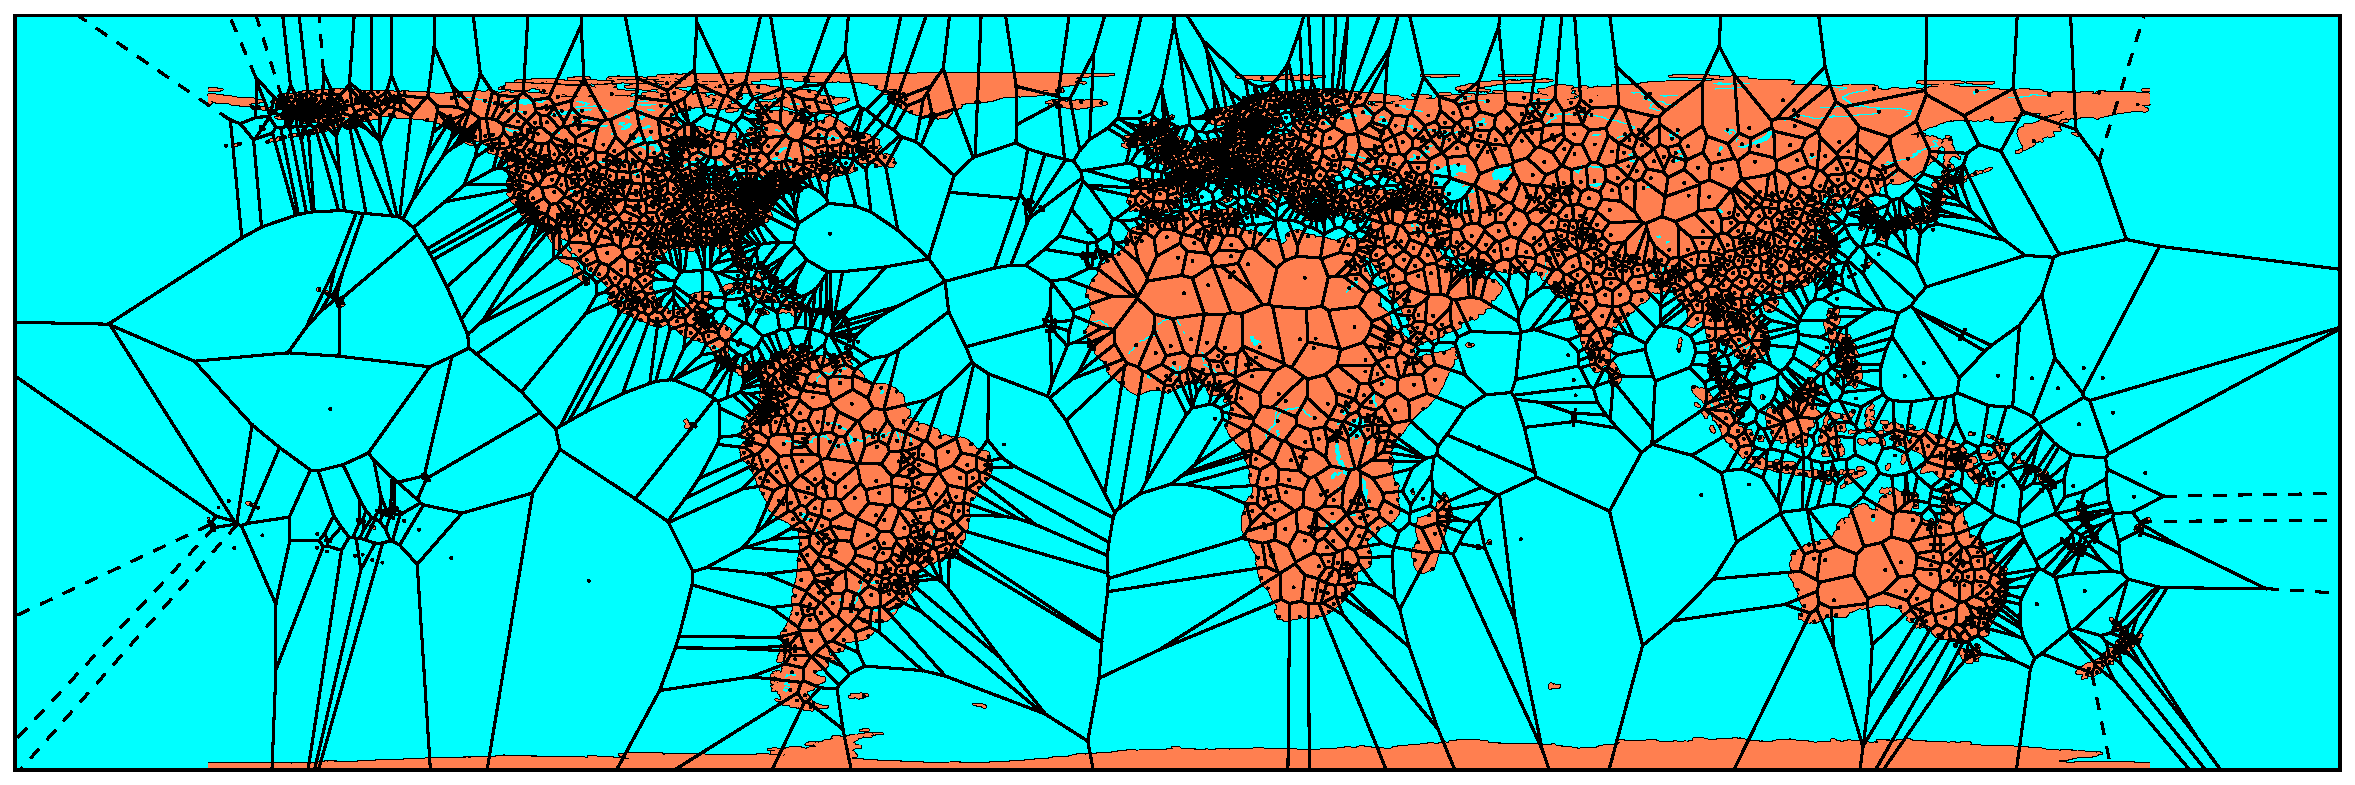
\includegraphics[width=1.0 \textwidth]{plots/voronoi.pdf}
	\caption{Voronoi tesselation based on airport locations. Airports are marked with a dot, region boundaries with lines and dashed lines.}
\end{figure}


%!TEX root = main.tex
\section{Modelling}
This report seeks to model the infection as a function of time of a global virus outbreak. To do, firstly it will be described how one might model a virus outbreak in small uniform population. Secondly, this model will be expanded to include multiple population groups and their interactions.

\subsection{The SIR Model}
\subsubsection{Assumption}
The Susceptible-Infected-Removed model is a compartmental model assuming that within some subdivision of the population containing $N$ individuals, virus infection, cure and spread rates are i.i.d. for the 3 ``compartments'' of individuals:
\begin{itemize}
	\item Susceptible to the virus
	\item Infected by the virus
	\item Recovered and immune to the virus (or alternatively dead)
\end{itemize} 
. In reality economic status, job type, air-conditioning etc. will affect how a virus spread \cite{zika-modelling}, however, depending on the heterogeneity of the population these assumptions constitute a good approximation.

\subsubsection{Governing equations}
The SIR model is governed by 3 differential equations,
\begin{align}
\frac{d S(t)}{dt} &= - \frac{\beta}{N} I(t) S(t)   \label{eq-S}\\
\frac{d I(t)}{dt} &= \frac{\beta}{N} I(t) S(t) - \gamma I(t)  \label{eq-I}\\
\frac{d R(t)}{dt} &= \gamma I(t) \label{eq-R}
\end{align}
where $S(t), I(t)$ and $R(t)$ are functions describing the number of susceptible, infected and removed individuals at time t, $\beta$ is the rate of infection, $\gamma$ the rate of removal (dead or cured) and $N$ the total number of individuals.

From equation \eqref{eq-S} and \eqref{eq-I} one can see that susceptible individuals become infected by some ratio $\beta$ and the ratio of already infected individuals. From \eqref{eq-I} and \eqref{eq-R} one can see that infected individuals recover with a constant factor $\gamma$. 

\begin{figure}[H]
	\centering
	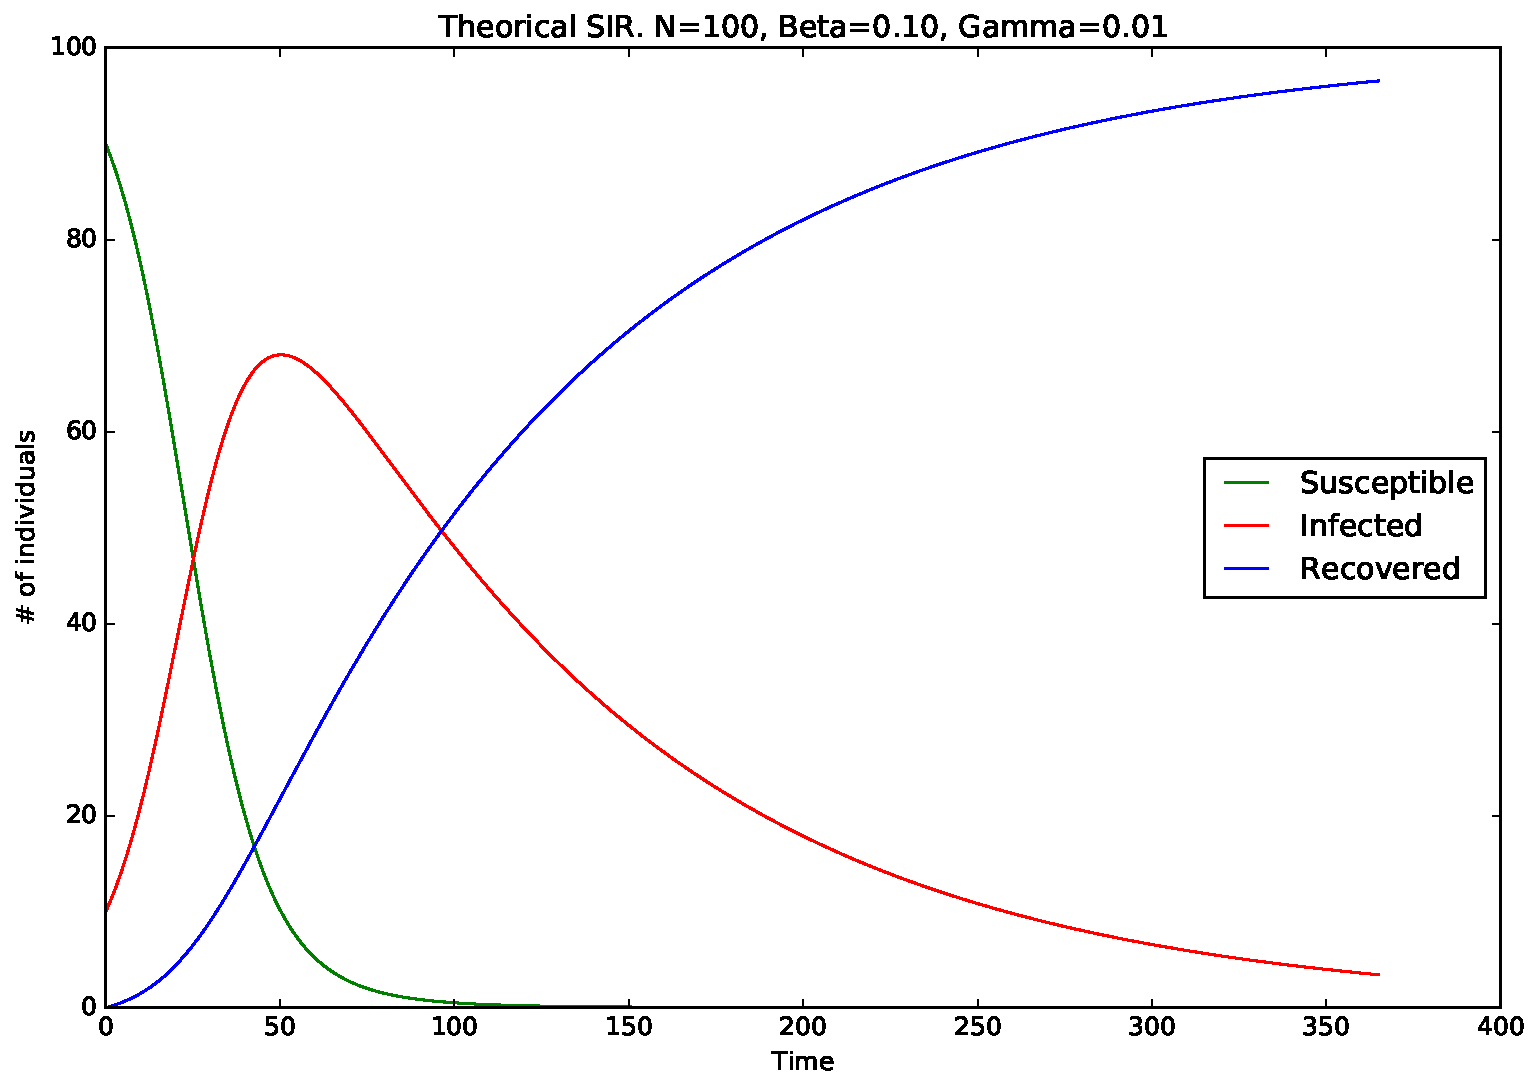
\includegraphics[width= 1.0 \linewidth]{plots/sir_one_region.pdf}
	\caption{Numerical solution to the nonlinear ODE system defining the SIR model.}
\end{figure}
\todo{comment on shape/interpretation of curve}

\subsection{Multi-region SIR}
Let it now be given that instead of having a single population, one has $K$ populations each with initial $N_k(0), S_k(0), I_k(0)$ and $R_k(0)$. Each of these populations have a probability of transferring individuals to other populations regardless of whether the individual is susceptible, infected or recovered. The governing equations are modified to add the transfers and become
\begin{align}
\frac{d S_k(t)}{dt} &= - \frac{\beta}{N_k} I(t) S(t) + \sum_{i\in K} \left( S_i(t)\tau_{i,k} - S_k(t)\tau_{k, i}\right)   &\forall k\\
\frac{d I_k(t)}{dt} &= \frac{\beta}{N_k} I(t) S(t) - \gamma I(t) + \sum_{i\in K} \left( I_i(t)\tau_{i,k} - I_k(t)\tau_{k, i}\right)  &\forall k\\
\frac{d R_k(t)}{dt} &= \gamma I(t) + \sum_{i\in K} \left( R_i(t)\tau_{i,k} - R_k(t)\tau_{k, i}\right) &\forall k
\end{align}
, where $\tau_{i,j}$ is the infinitesimal probability of transferring from population $i$ to $j$ per individual.

As an example of the above system let $K=3$ and the non zero transfer probabilities be defined by the graph:
\begin{figure}[H]
	\centering
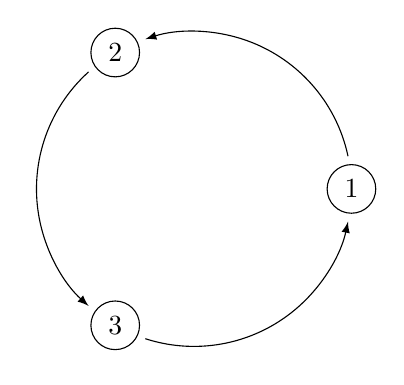
\begin{tikzpicture}

\def \n {3}
\def \radius {2cm}
\def \margin {12} % margin in angles, depends on the radius

\foreach \s in {1,...,\n}
{
	\node[draw, circle] at ({360/\n * (\s - 1)}:\radius) {$\s$};
	\draw[->, >=latex] ({360/\n * (\s - 1)+\margin}:\radius) 
	arc ({360/\n * (\s - 1)+\margin}:{360/\n * (\s)-\margin}:\radius);
}
\end{tikzpicture}
\end{figure}
. Solving this system numerically with the outbreak starting in region 1 one gets the following curves:
\begin{figure}[H]
	\centering
	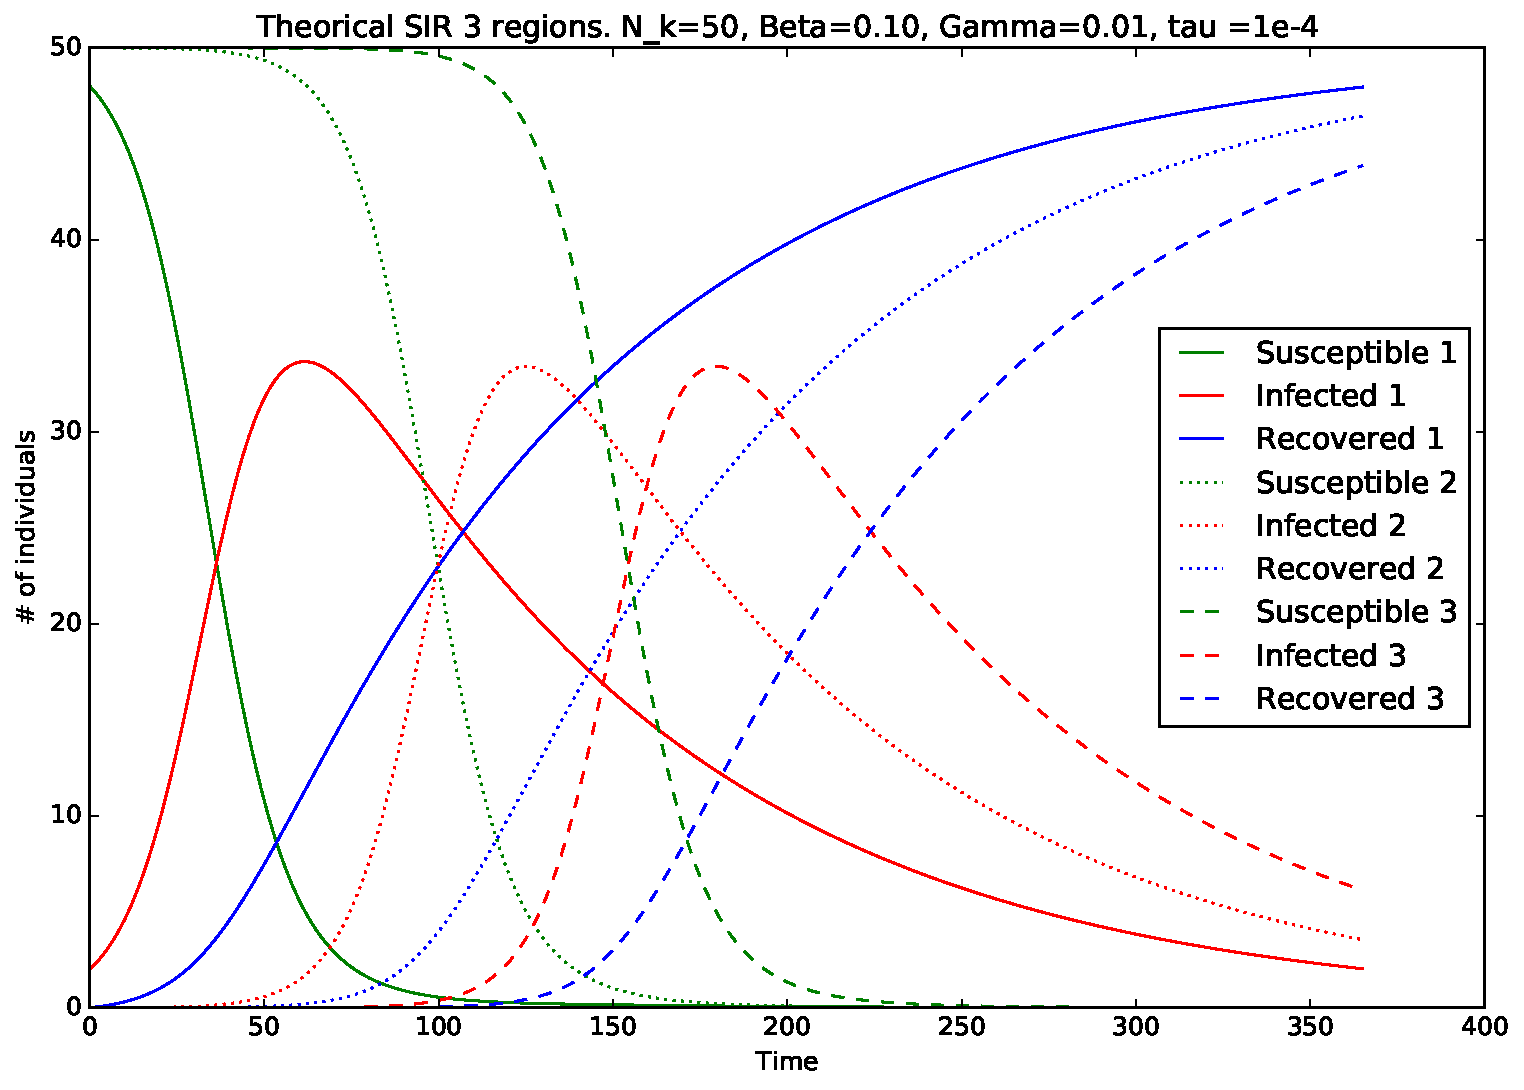
\includegraphics[width= 1.0 \linewidth]{plots/sir_three_region.pdf}
	\caption{Numerical solution to the nonlinear ODE system defining a 3-region SIR model.}
\end{figure}

From the above plot it's seen that the virus first spreads in region 1. After a certain time a enough infected individuals have been transferred to region 2 where the infection then accelerates. This continues to region 3.

\subsection{}

\subsection{Stocastic Model}

To simulate the multi-region SIR model stochastically, a binomial distribution is used to sample how many people get infected, removed and transferred. The binomial probability is chosen such the expectation is the same, as in the differential equation model.
\begin{equation*}
\begin{aligned}
\Delta I_{k,t} &= \textsc{Binom}\left(S_{k,t}, \beta \frac{I_{k, t}}{N_k}\right) \\
\Delta R_{k,t} &= \textsc{Binom}\left(I_{k,t}, \gamma\right) \\
S_{k,t} &= S_{k,t-1} - \Delta I_{k,t} + \sum_{i \in K} \left(\textsc{Binom}(S_{i,t-1}, \tau_{i,k}) - \textsc{Binom}(S_{k,t-1}, \tau_{k,i})\right) \\
I_{k,t} &= I_{k,t-1} + \Delta I_{k,t} - \Delta R_{k, t} + \sum_{i \in K} \left(\textsc{Binom}(I_{i,t-1}, \tau_{i,k}) - \textsc{Binom}(I_{k,t-1}, \tau_{k,i})\right) \\
R_{k,t} &= R_{k,t-1} + \Delta R_{k, t} + \sum_{i \in K} \left(\textsc{Binom}(R_{i,t-1}, \tau_{i,k}) - \textsc{Binom}(R_{k,t-1}, \tau_{k,i})\right)
\end{aligned}
\end{equation*}

where $\tau_{i,j}$ now is the discretized transfer probability.

\subsubsection{Transfer using Dirichlet distribution}
A problem with this approach, is the small risk that $\textsc{Binom}(S_{i, t-1}, \tau_{i,k}) = 0$ and $\textsc{Binom}(S_{k, t-1}, \tau_{k,i}) = S_k$ or similar unfortunate combination which will cause $S_{k,t}$ to become negative. This turns out to be a practical problem, to avoid this problem one should sample all the transfers for a region simultaneously such $\sum_{i \in K} \textsc{Binom}(S_{k,t-1}, \tau_{k,i}) \le S_{k, t}$.

As there does not exist a multivariate version of the binomial distribution, the Dirichlet distribution is used as an approximation. This is convenient because $\sum_{i} X_{i,k} = 1$ if $\mathbf{X}_k \sim \textsc{Dir}(\boldsymbol{\alpha}_k)$. Because the Dirichlet distribution has support $X_i \in [0, 1]$, $\floor*{N_k X_{i,k}}$ is used.

Furthermore to reduced the amount of sampling, the total transfer $T$ is sampled instead of sampling $S$, $I$ and $R$ independently.

To approximate the binomial distribution using a Dirichlet distribution the expectation is set to be the same. To simplify notation region $k$ is omitted from the subscript and the summarization of $tau_k$ and $\alpha_i$ is introduced:
\begin{equation}
\tau_s = \sum_{k = 1}^{K} \tau_k, \quad \alpha_s = \sum_{k = 1}^{K+1} \tau_k
\end{equation}

\begin{equation}
\mathbb{E}[T_{i}] = \mathbb{E}[N X_i] \Leftrightarrow N \tau_i = N \frac{\alpha_i}{\alpha_s} \quad \forall i \in K
\label{dir-expected-trans}
\end{equation}

To allow $\sum_{i} X_{i,k} \le 1$ the Dirichlet distribution is extended with another variable $X_{k, K+1}$, which will be how large a proportion region $k$ should keep.
\begin{equation}
\mathbb{E}[T_{K+1}] = \mathbb{E}[N X_{K+1}] \Leftrightarrow N \left(1 - \tau_s\right) = N \frac{\alpha_{K+1}}{\alpha_s}
\label{dir-expected-stay}
\end{equation}
  
This is a linear system with n variables and n equations, but it turns out not to have full rank. To add another equation the variance of $T_{K+1}$ is also set to be the same.
\begin{equation}
\textsc{Var}[T_{K+1}] = \textsc{Var}[N X_{K+1}] \Leftrightarrow N\tau_s (1 - \tau_s) = N^2 \frac{\alpha_{K+1}(\alpha_s - \alpha_{K+1})}{\alpha_s^2 (\alpha_s + 1)}
\label{dir-var}
\end{equation}

The trick to solving this set of equations, is to isolate $\alpha_s$ from \eqref{dir-expected-stay} and insert it into \eqref{dir-expected-trans} and \eqref{dir-var}.
\begin{align}
\alpha_s &= \frac{\alpha_{K+1}}{1 - \tau_s} \label{dir-expected-intermediate} \\
N \tau_i &= N \frac{\alpha_i}{\frac{\alpha_{K+1}}{1 - \tau_s}} \quad \forall i \in K \\
N\tau_s (1 - \tau_s) &= N^2 \frac{\alpha_{K+1}\left(\frac{\alpha_{K+1}}{1 - \tau_s} - \alpha_{K+1}\right)}{\left(\frac{\alpha_{K+1}}{1 - \tau_s}\right)^2 \left(\frac{\alpha_{K+1}}{1 - \tau_s} + 1\right)} \label{dir-var-intermediate}
\end{align}

$\alpha_{K+1}$ can now be isolated from \eqref{dir-var-intermediate} yielding
\begin{equation}
\alpha_{K+1} = (N - 1) - \tau_s (N - 1)
\end{equation}
, inserting this into \eqref{dir-expected-intermediate} gives:
\begin{equation}
\alpha_{i} = \tau_i (N - 1)
\end{equation}
Using the $\alpha_{i}$ solution $\alpha_{K+1}$ can now be reformulated as
\begin{equation}
\alpha_{K+1} = (N - 1) - \sum_{i=1}^K \alpha_k
\end{equation}
which is computationally slightly more convenient.

Using this method for choosing $\alpha$, gives the distribution as seen in Figure\ref{fig:dirichlet-validation}. As seen it has only minor errors when comparing to the binomial distribution.

\begin{figure}[H]
	\centering
	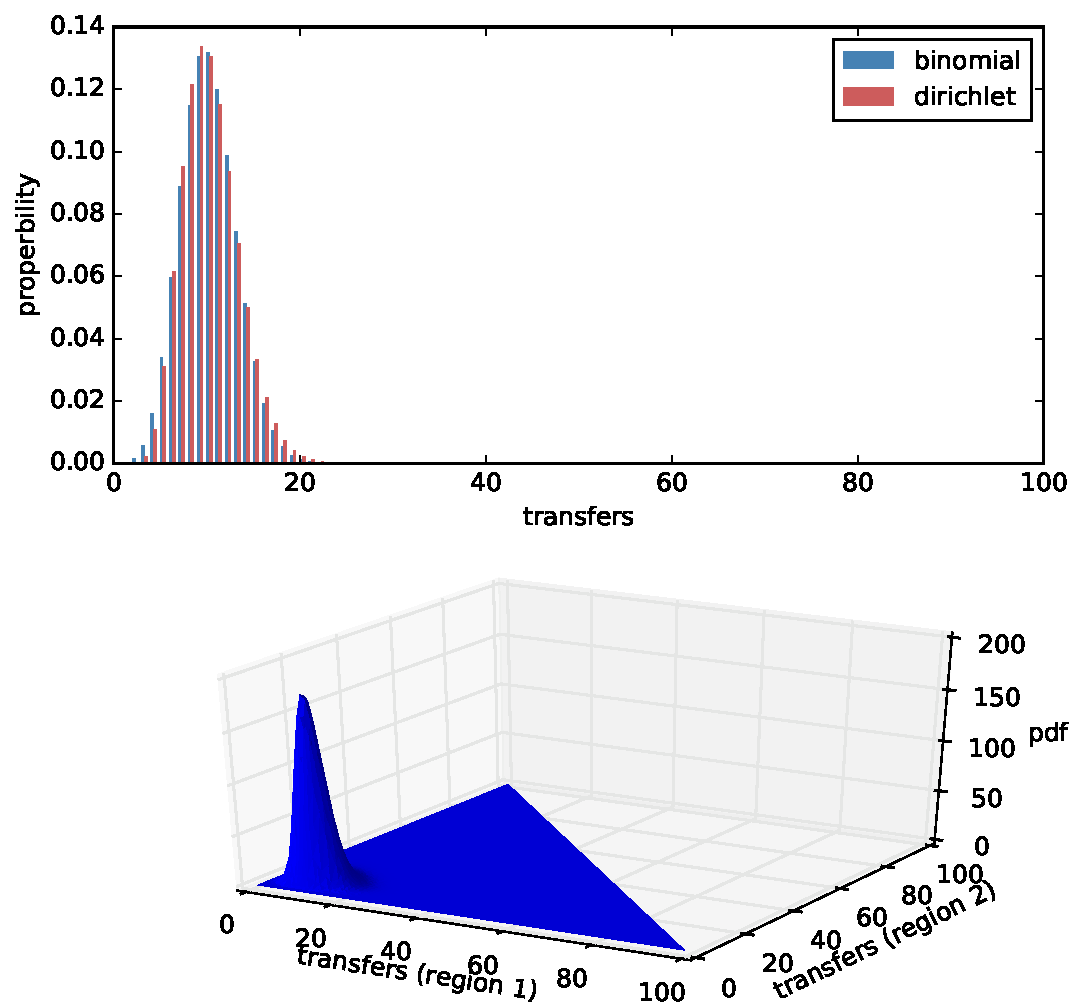
\includegraphics[width= 1.0 \linewidth]{plots/dirichlet-validation}
	\caption{A dirichlet distribution  upscaled by $N$, with $\tau = (0.1, 0.1)$ and $N = 100$. First figure compare the marginal probability $P(\floor*{N X_1})$ with the binomial distribution. Second figure shows the Dirichlet pdf with $X_3 = 1- X_1 - X_2$.}
	\label{fig:dirichlet-validation}
\end{figure}


\section{Validation}

To validate our implementation of the stochastic simulation model, the 3 region problem previously solved using differential equations, is now solved using the stochastic model.

\begin{figure}[H]
	\centering
	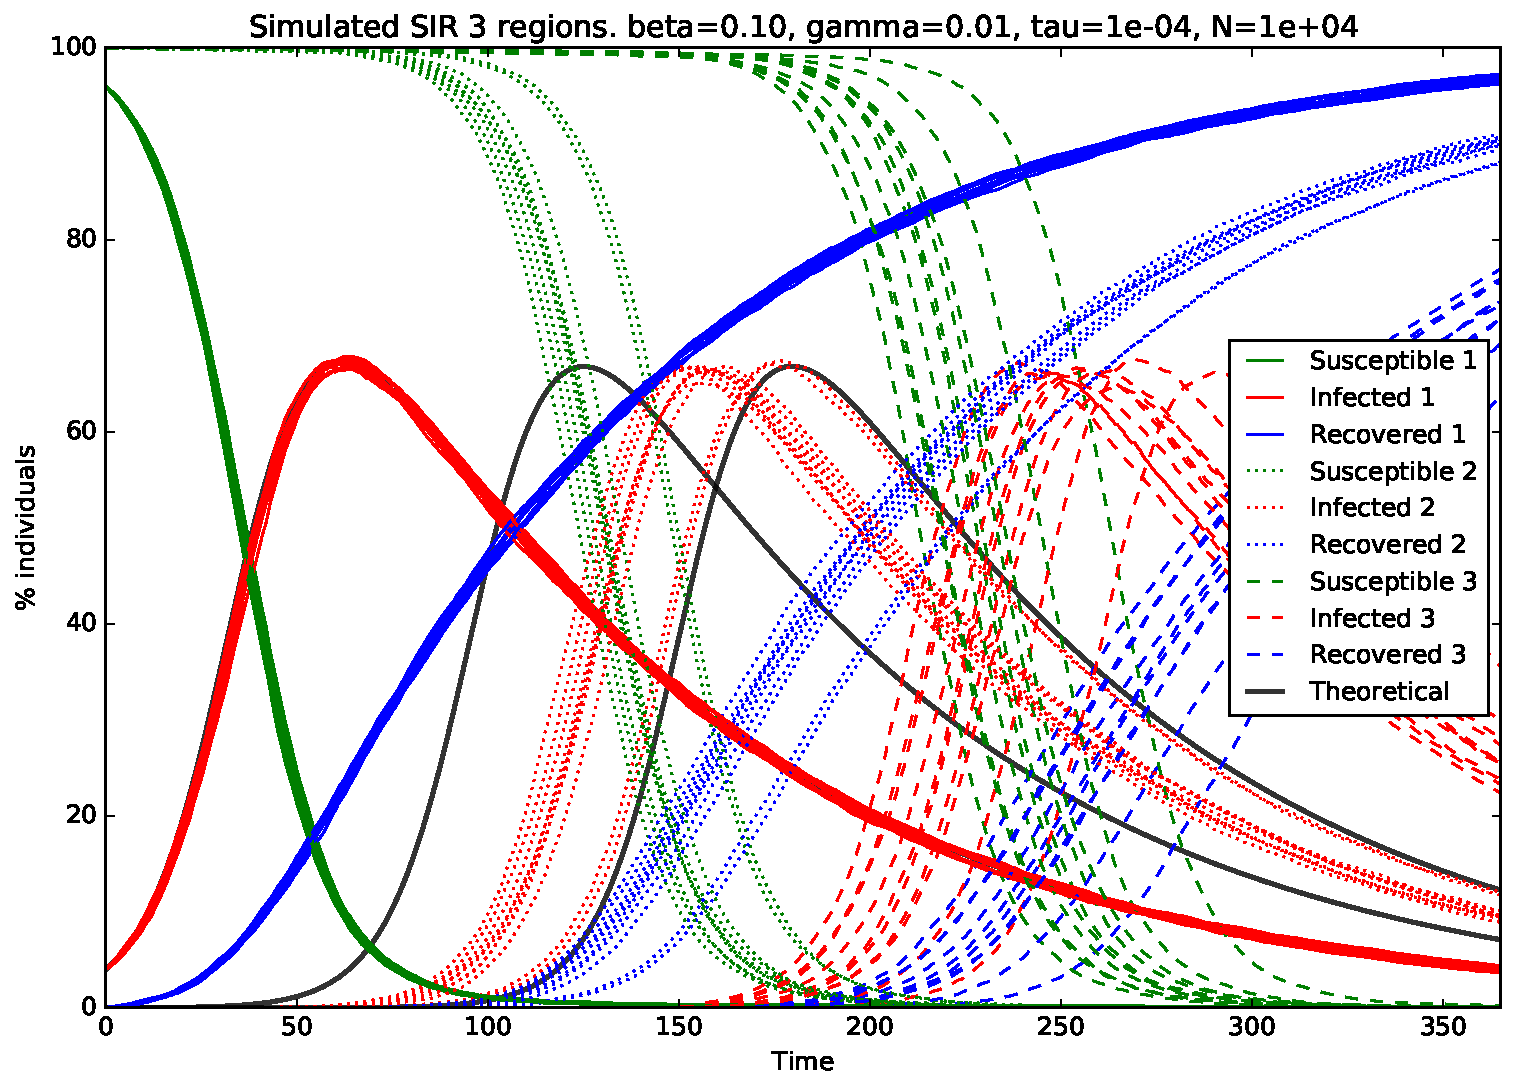
\includegraphics[width= 1.0 \linewidth]{plots/sir_three_region_sim_10000.pdf}
	\caption{10 solutions using the stochastic simulation model, on the same 3-region problem as in the theoretical case.}
	\label{fig:sir_three_region_sim_10000}
\end{figure}

Figure \ref{fig:sir_three_region_sim_10000} shows a big discrepancy between the solution obtained using differential equations and the those obtained using stochastic simulation. This is most likely because the differential equation model allows for transferring people partially, . This means regions that has a very low probability of getting infected early in the stochastic model, starts their infection immediately in the differential equation model. This hypothesis can be validated by increasing the number of people in each region (N), as this will cause the discreteness of the stochastic model to be less important. The result of this can be seen in figure \ref{fig:sir_three_region_sim_1000000}. 

\begin{figure}[H]
	\centering
	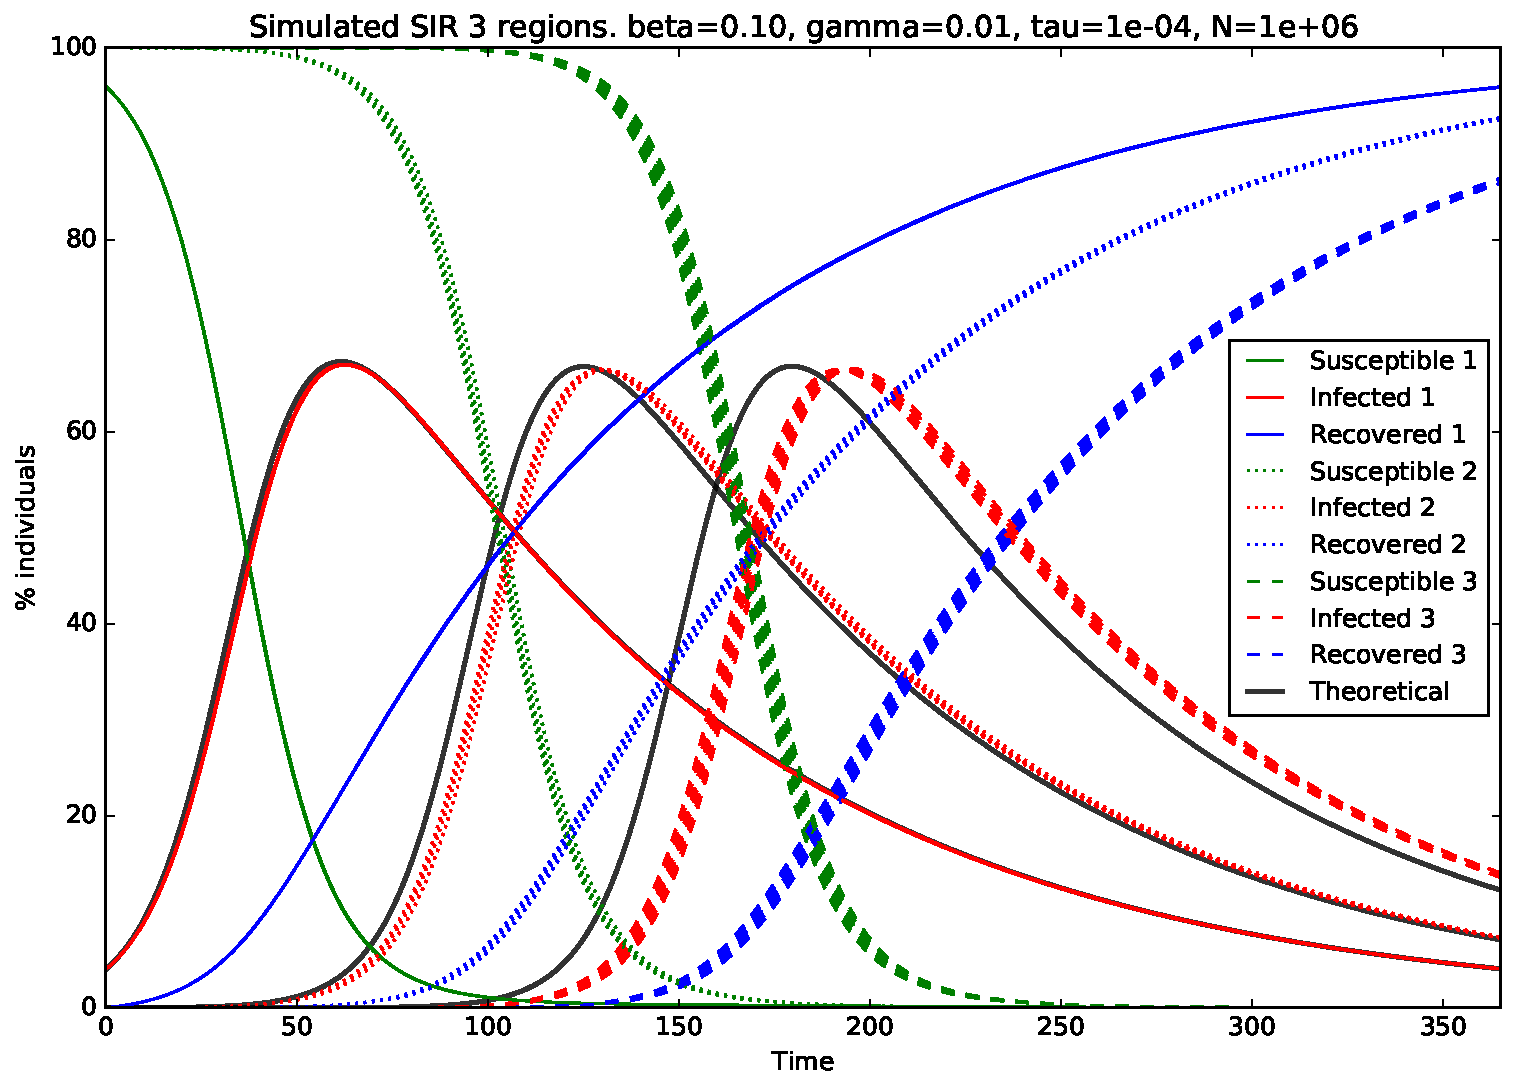
\includegraphics[width= 1.0 \linewidth]{plots/sir_three_region_sim_1000000.pdf}
	\caption{10 solutions using the stochastic simulation model, on the same 3-region problem as in the theoretical case.}
	\label{fig:sir_three_region_sim_1000000}
\end{figure}

As seen in figure \ref{fig:sir_three_region_sim_1000000} having more people results a much smaller discrepancy. This discrepancy caused by using a discrete model is not necessarily a failure of the stochastic model, but rather it is the differential equation model that overestimates the infection start for initially healthy regions.

%!TEX root = main.tex
\section{Simulation setup}
\subsection{Variance reduction}
Because the simulation can be time consuming to run, we want to lower the variance of the estimated parameters as much as possible relative to the computational resources used.

\subsubsection{Control Variates}
Control variates is a variance reduction technique which can be used to reduce the variance of the estimated expected value $\hat{\mu} = \mathbb{E}[Y]$. It works by drawing/calculating a variable $X_i$ such that $Y_i \approx f(X_i)$. One can then estimate $\hat{\mu} = \mathbb{E}[Z]$ where $Z$ is given by:
\begin{align}
Z_i = Y_i - c (X_i - \mathbb{E}[X])
\end{align}

Choosing $c = \frac{Cov(X, Y)}{Var(X)}$ gives the largest variance reduction of:
\begin{equation}
\frac{Var[Z]}{Var[Y]} = \frac{Var[Y]}{Var[Y]} - \frac{Cov(X, Y)^2}{Var[X] Var[Y]} = 1 - \rho_{x, y}^2 \label{eq:variance-reduction}
\end{equation}

In our case there is no analytical expression for the covariance or variance of the random variables. Instead $c$ is estimated from the dataset itself. This introduces some overfitting, thus one should take care to reduce the degrees of freedom in the variance, covariance estimates:
\begin{equation}
\hat{c} = \frac{Cov_{N-1}(X, Y)}{Var_{N-1}(X)}, \quad \hat{\sigma}^2 = Var_{N-2}(Z)
\end{equation}

The subscript denotes the degrees of freedom, and $\hat{\sigma}^2$ has $N - 2$ degrees of freedom, because $\hat{c}$ is estimated from the dataset.

\subsubsection{Estimating infection rate}

From \eqref{eq:variance-reduction} it seen that to get a high variance reduction, $X_i$ just need to be heavily correlated with $Z_i$. In our case we would like to estimate the infection peak time and how many people where infected at the peak. From the theoretical differential equation model those values should be correlated with the infection rate $\beta$.

Assuming the stochastic model have a behaviour somewhat similar to the differential equation model, there exists fairly simple methods for estimating $\beta$ and $\gamma$ \cite{wiki-sir}.
\begin{equation}
\gamma = \frac{R'_{max}}{I_{max}} \text{ and } \beta = -\frac{\ln(p)}{1 - p} \gamma \quad \text{where: } p = \frac{N - R_\infty}{N} 
\end{equation}

$R'_{max}$ is the maximum removed difference, and $I_{max}$ is the maximum infected. Due to the construction of the differential equation, these are found at the same time $t$. $R_\infty$ is how many people where removed in the end, thus $p$ is the survival rate.

\subsection{Effect of Global Events}
We want to estimate what effect a global event can have on a virus outbreak. We define an event $e$ as simply being a transfer of people from one or more regions $r_{i}$ to region $r_t$ at a time $t_0$, and the reverse transfer of people from $r_t$ to $r_{i}$ at time $t_1$.

\subsubsection{Motivation: Zika virus}
Recently, a new virus has been observed in South and Latin America. The Zika virus affects pregnant women's fetuses and can cause serious birth defects. The Zika virus is primarily spread by mosquitoes, but can also spread from a man to his sex partners (and from mother to fetus). Some political discussions have been made as to whether or not the Olympic Games should be canceled to prevent the spreading of the virus.

In this report we will run a "hypothetical" simulation, showing how the a virus could spread assuming inter-human infections. As such this simulation is primarily an attempt of showing how such a model would work and not a realistic Zika virus predictor.

\subsubsection{Event definition: Olympic Games in Rio 2016}
In our simulation we define the Olympic Games to take place during $t_0=$ `2016-07-03' and $t_1=$ `2016-07-21'. According to The Gaurdian \cite{theguardian-olympics} Rio expects to recieve 380,000 tourist. We choose to transfer people from all over the world to Rio, such that the transfer is proportional to the population size of each region:

\begin{align}
	\text{Transfer}_0(i, j) &= 380000 \cdot \frac{\text{population}_i}{N} \\
	\text{Transfer}_1(j, i) &= \text{transfer}_0(i, j)
\end{align}

where $\text{Transfer}_0(i, j)$ denotes the number of people transferred from region $i$ to region $j$ at the start of the Olympics and $ \text{Transfer}_1(j, i) $ the people transferred from $j$ to $i$ at the end of the Olympics.

%!TEX root = main.tex
\section{Results}
\subsection{With and without Olympic Games}
Choosing $\beta=2$, $\gamma=0.5$ and an average transfer probability of $0.005$ we can run a simulation with and without the Olympic Games occurring with the previously described characteristics. We assume that the infection breaks out on the first day of the games in Rio De Janeiro. We set the initial infected population to 1000. In the following we will look at the SIR curves of 6 major cities.

With the Olympics occurring we get the following curves:
\begin{figure}[H]
	\centering
	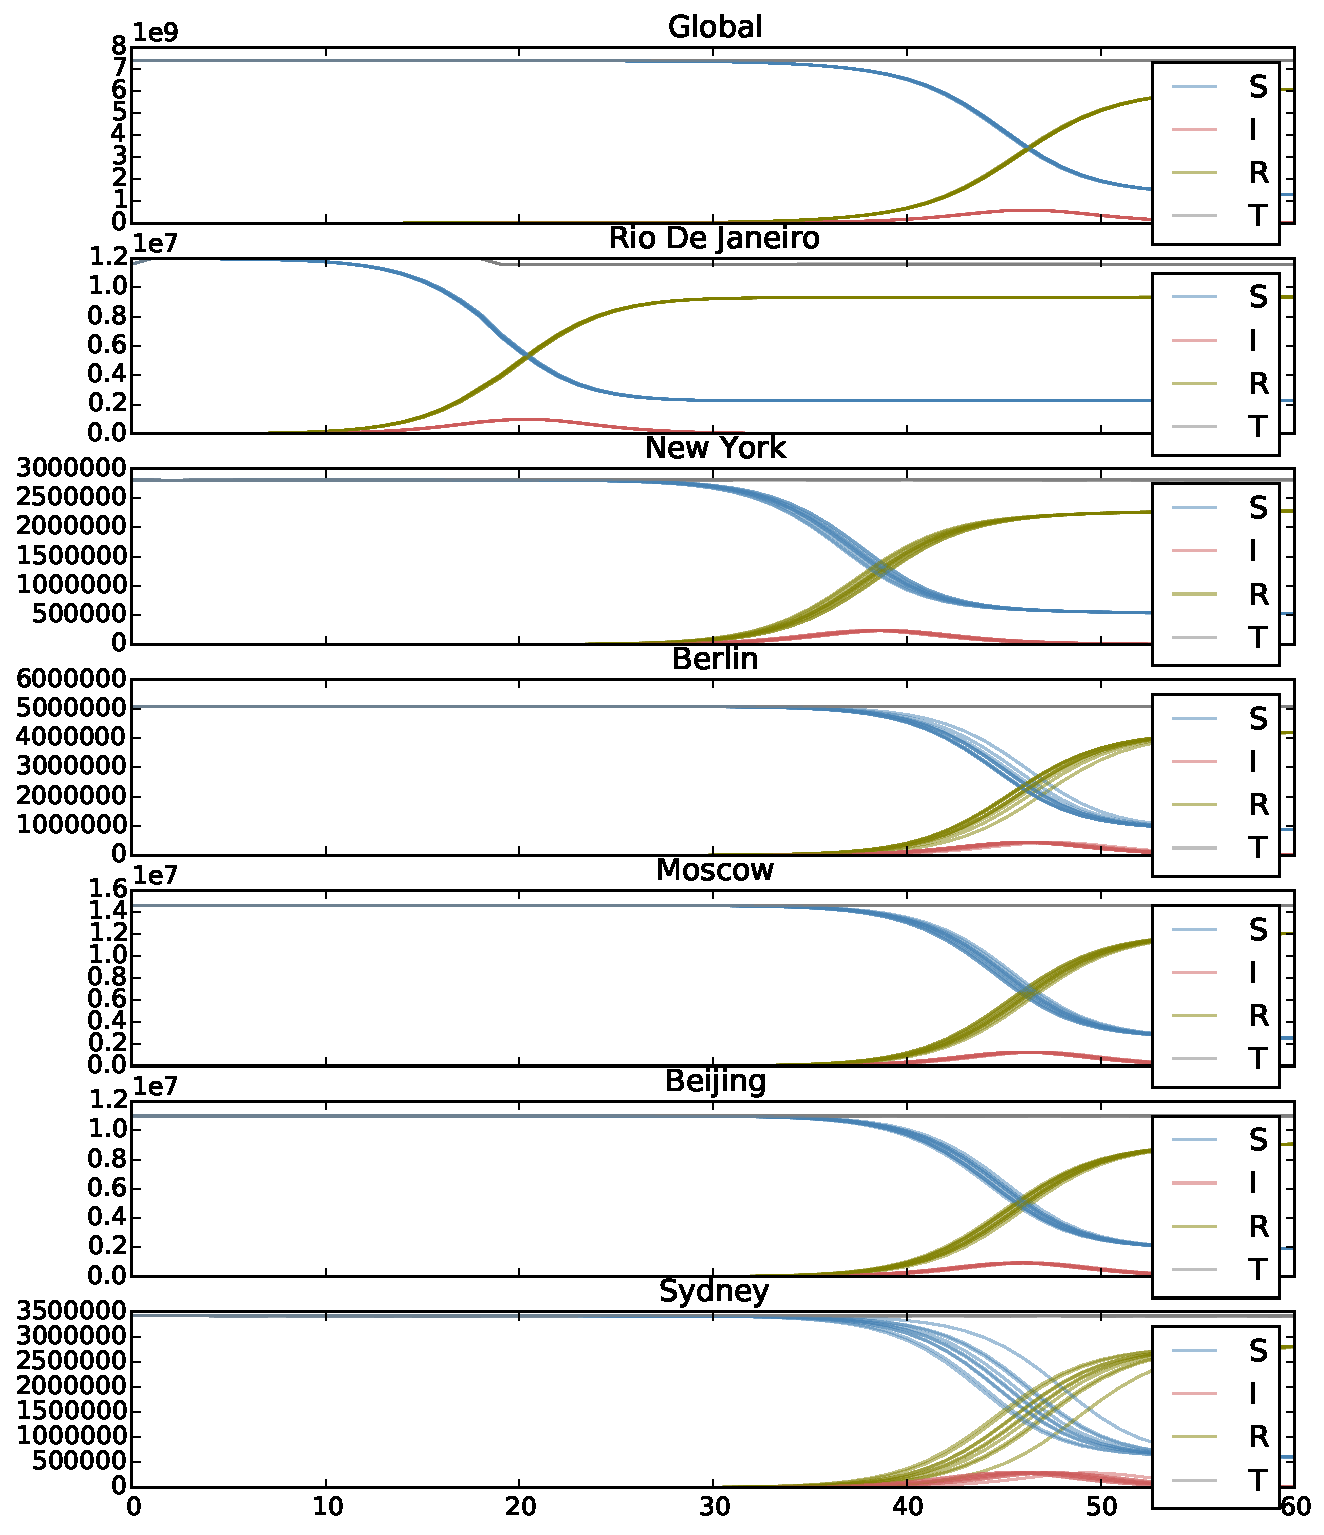
\includegraphics[width=1.0 \linewidth]{plots/rio-0-18-380000.pdf}
	\caption{10 simulations with Olympic Games. Time in days on the x-axis and number of people on the y-axis}
\end{figure}

From the above plot we see that except for New York which seems to be infected quickest, the other major cities all seem to reach peak infection rates at the same time. 

\begin{figure}[H]
	\centering
	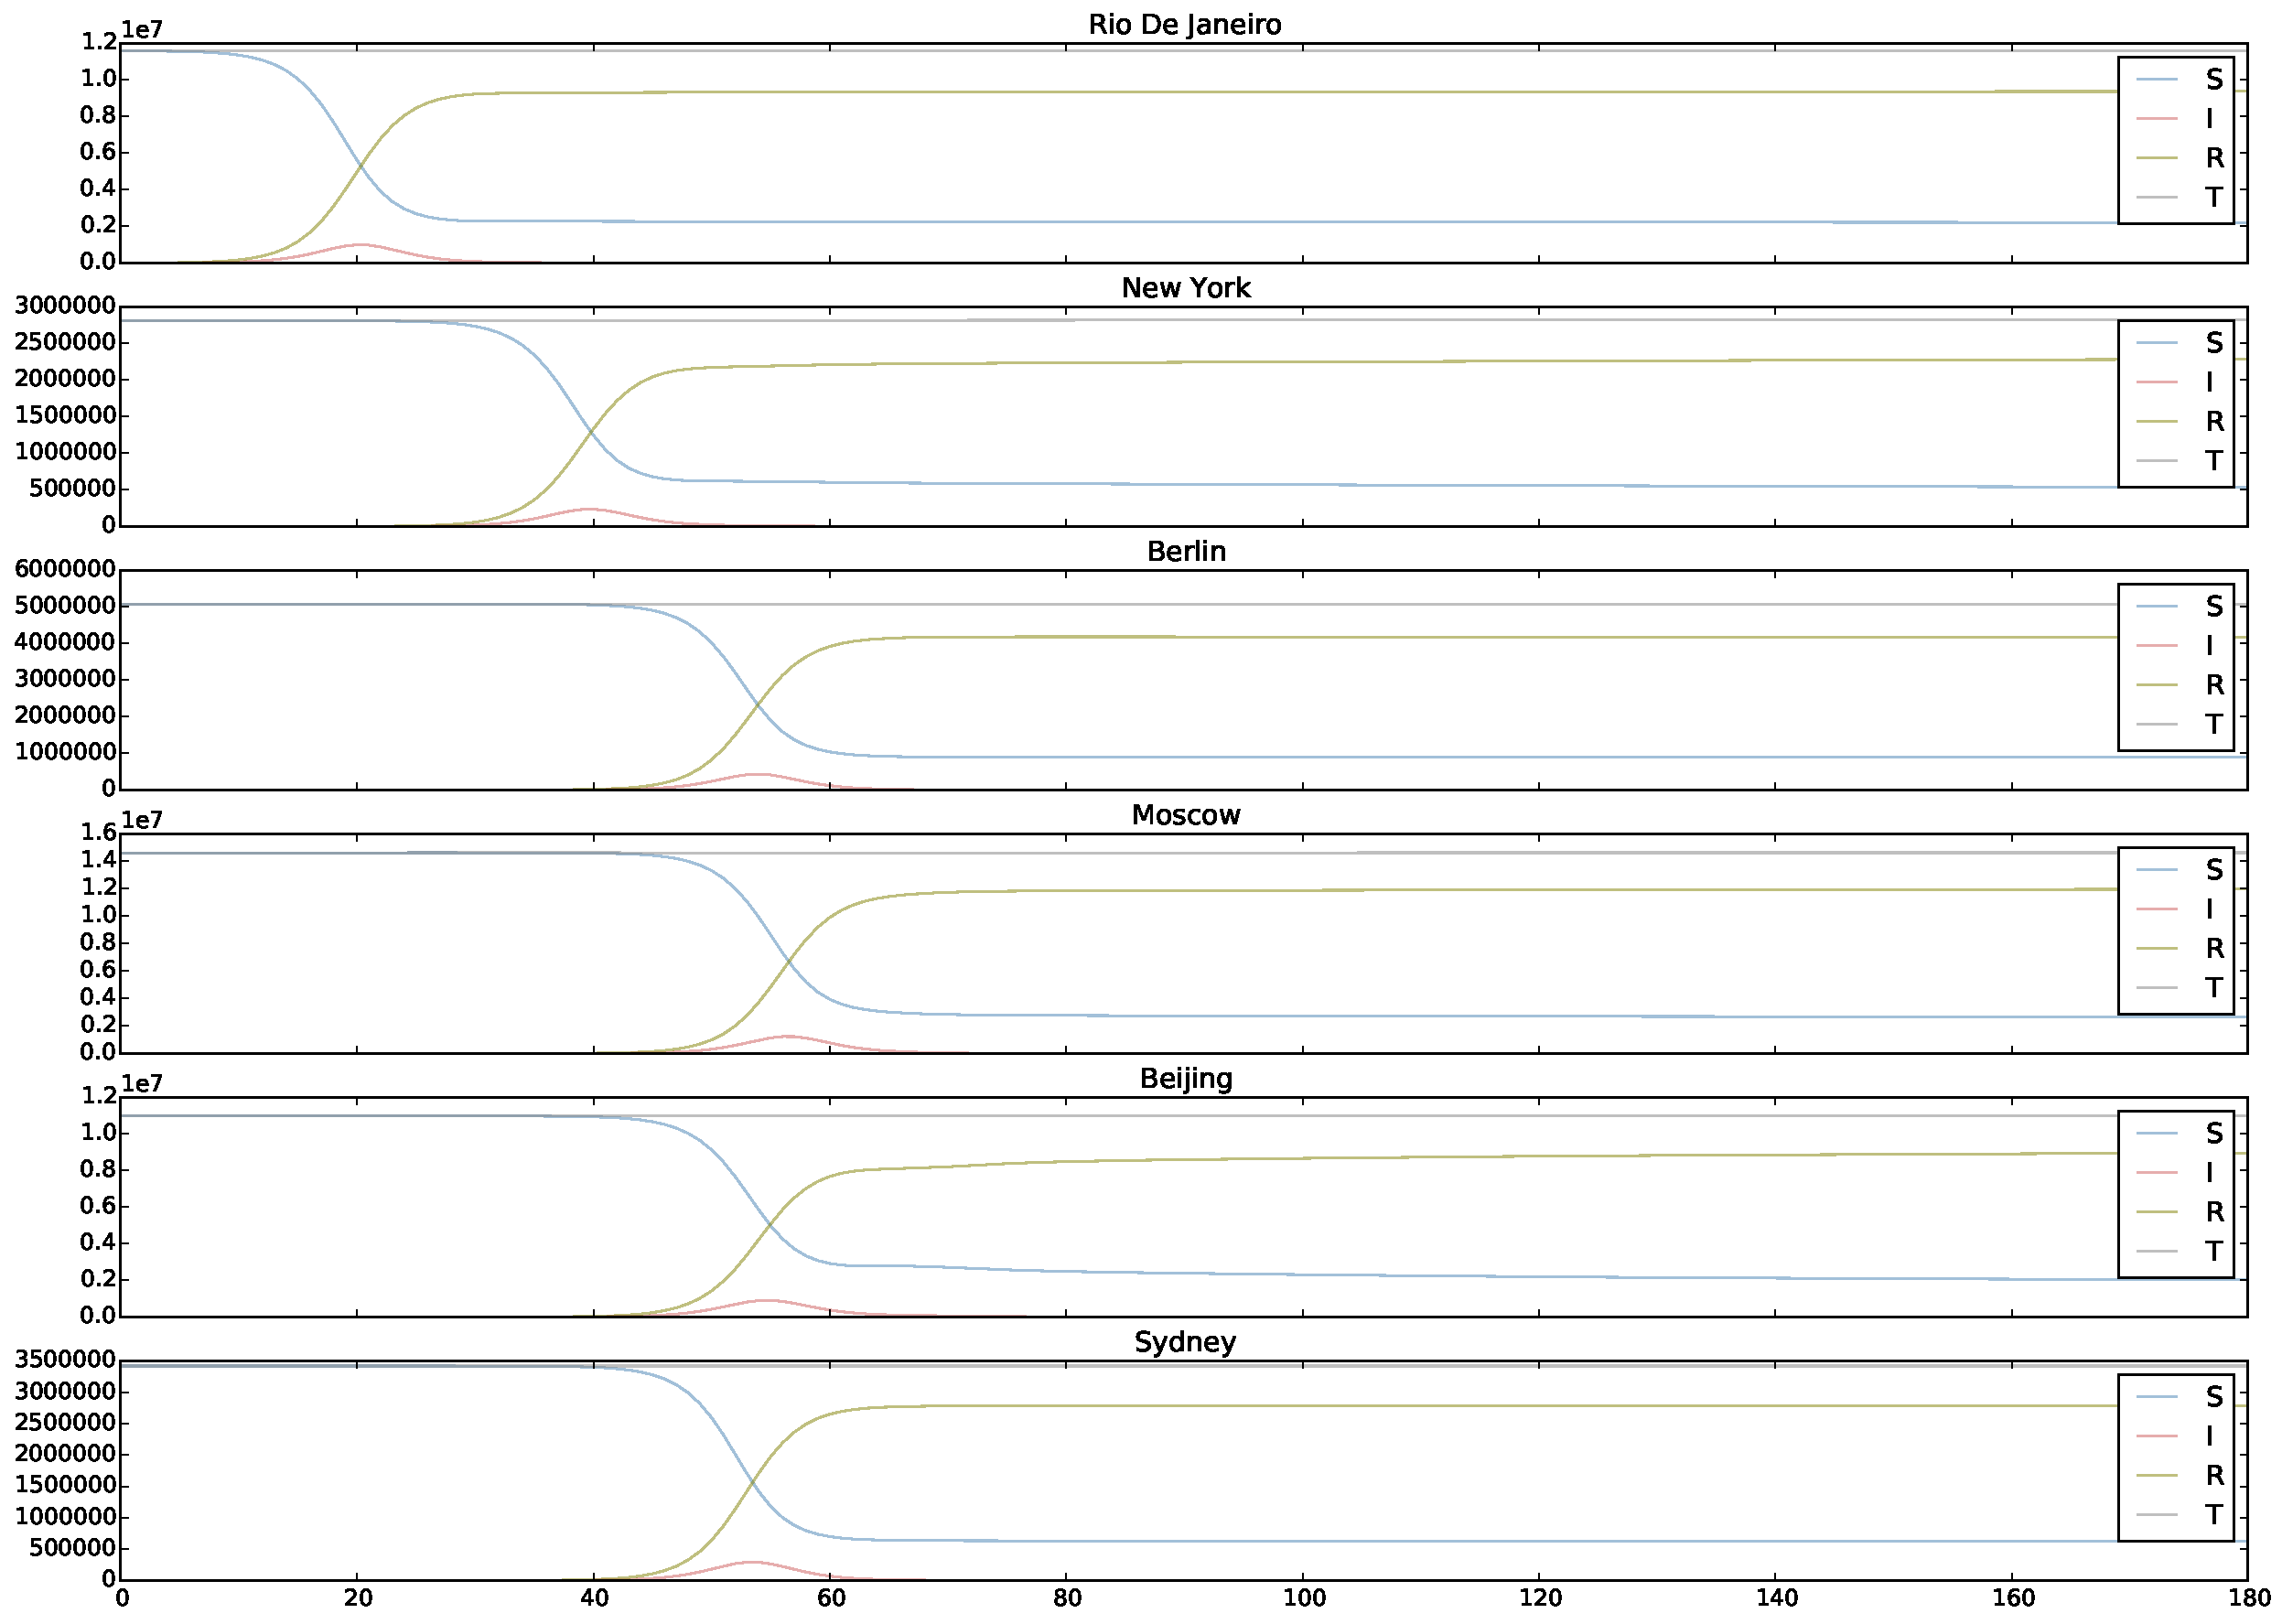
\includegraphics[width=1.0 \linewidth]{plots/no_rio.pdf}
	\caption{10 simulations without Olympic Games. Time in days on the x-axis and number of people on the y-axis}
\end{figure}

If one looks closely at the plot above we see that without the Olympic Games peak infections occur later for especially Moscow, Beijing and Sydney. The is perhaps a bit easier to see in the table below:

\begin{table}[H]
	\centering
	\begin{tabular}[H]{c | c | c}
Observation & With OL & Without OL \\ \hline 
 Peak amount Global [million]& $590.5\pm 0.94 (0.02)$ & $291.5 \pm 1.41 (0.01)$\\ 
 Peak time Global & $46.0\pm 0.00( 0.00)$ & $67.0 \pm 0.00 (0.00)$\\ 
 Peak time Rio & $20.2\pm 0.30( 0.26)$ & $20.0 \pm 0.00 (0.00)$\\ 
 Peak time New York & $38.6\pm 0.50( 0.52)$ & $38.3 \pm 0.59 (0.50)$\\ 
 Peak time Berlin & $46.4\pm 0.77( 0.56)$ & $53.7 \pm 0.35 (0.30)$\\ 
 Peak time Moscow & $46.1\pm 0.23( 0.23)$ & $56.3 \pm 0.35 (0.28)$\\ 
 Peak time Beijing & $46.0\pm 0.00( 0.00)$ & $55.0 \pm 0.34 (0.30)$\\ 
 Peak time Sydney & $46.3\pm 0.83( 0.73)$ & $53.3 \pm 0.48 (0.51)$
\end{tabular}
	\caption{Results of 10 simulations with and without Olympic Games. Table contains the peak times and amounts for the number of infected individuals. The standard $95\%$-confidence interval is marked with $\pm$ and the confidence interval using control variates is shown in the parenthesis.}
\end{table}]

\todo{comment on table}

\subsection{Visualization of result}
When studying a virus outbreak it is interesting to see exactly how the virus spreads. We have thus created an animation on a world map showing where each region is represented as a dot (scaled according to the population size) and the color of the dot represents the fraction infected. With this visualization the difference between including the Olympic Games and including becomes more apparent.

\begin{figure}[H]
	\centering
	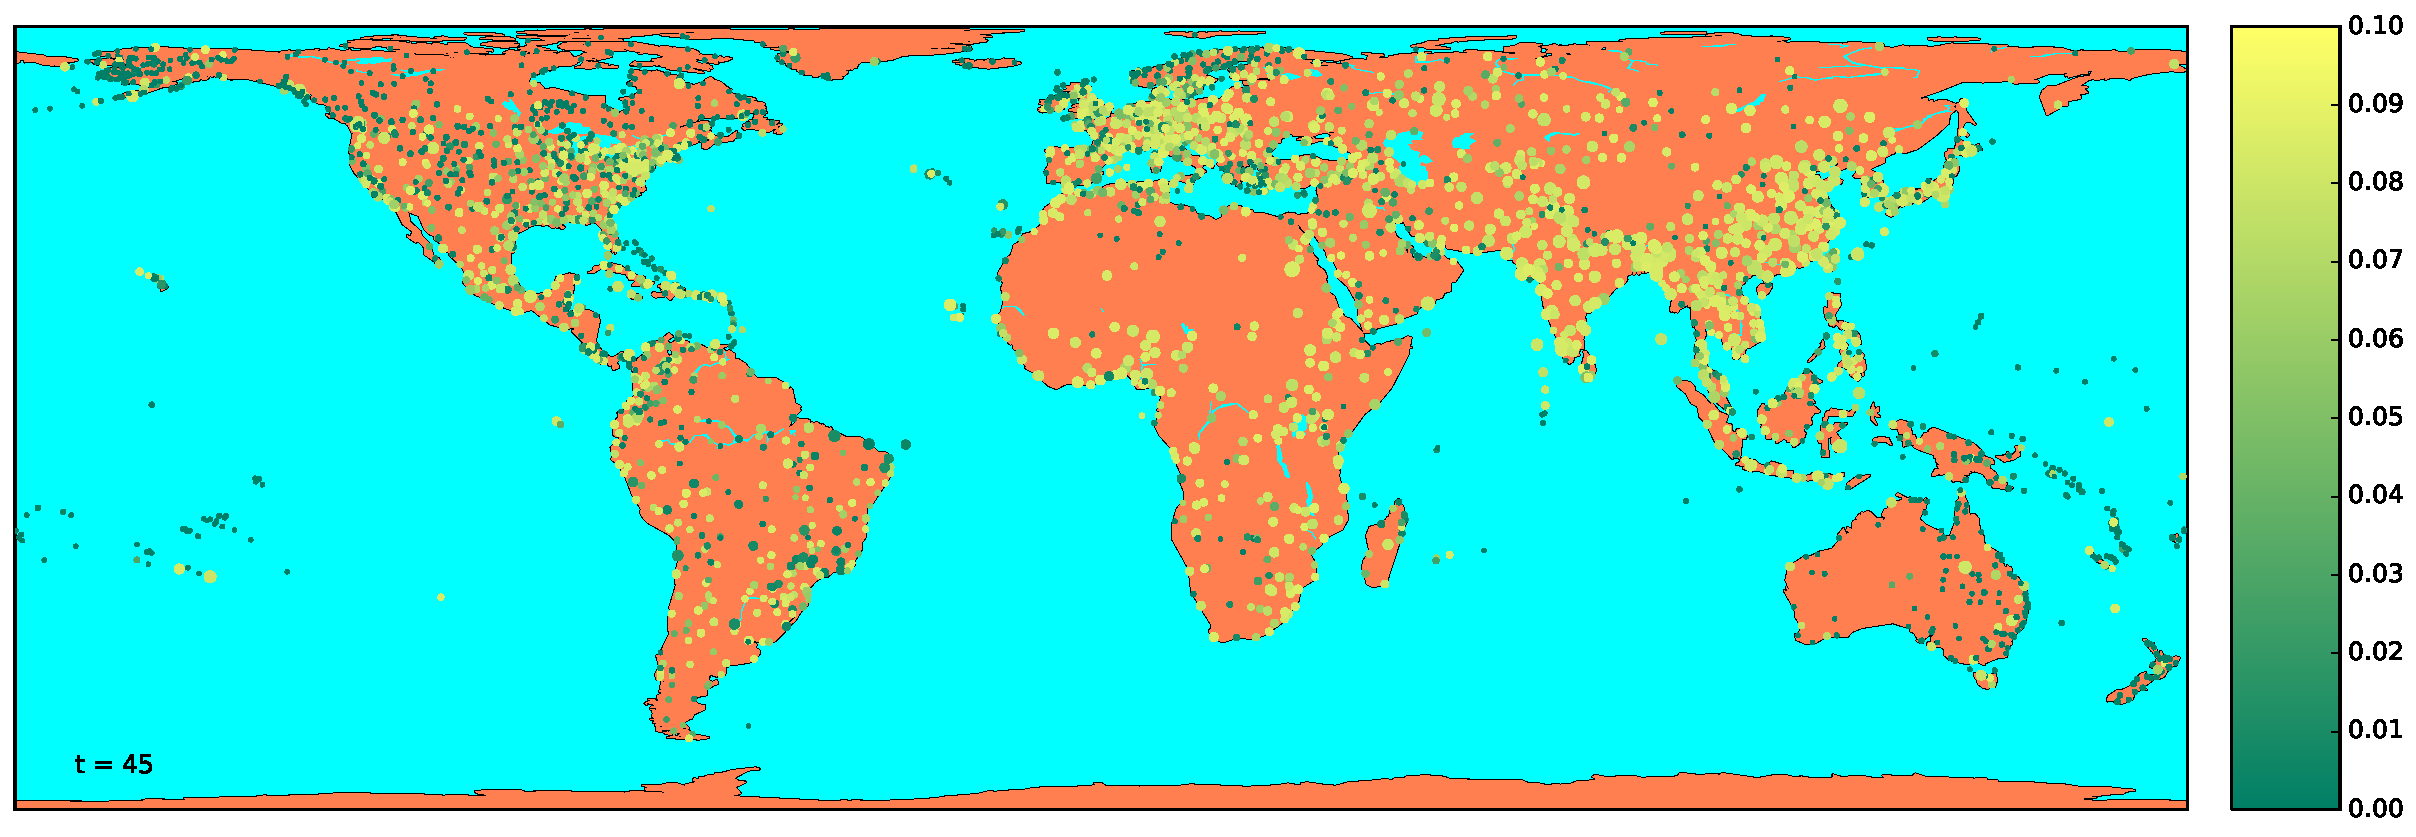
\includegraphics[width=1.0 \linewidth]{plots/gifs/frames/rio-45}
	\caption{Frame 45 of animation with Olympic Games. The full animation can be viewed as a gif at
		\url{https://andreasmadsen.github.io/course-02443-stochastic-virus-outbreaks/}}
\end{figure}

\begin{figure}[H]
	\centering
	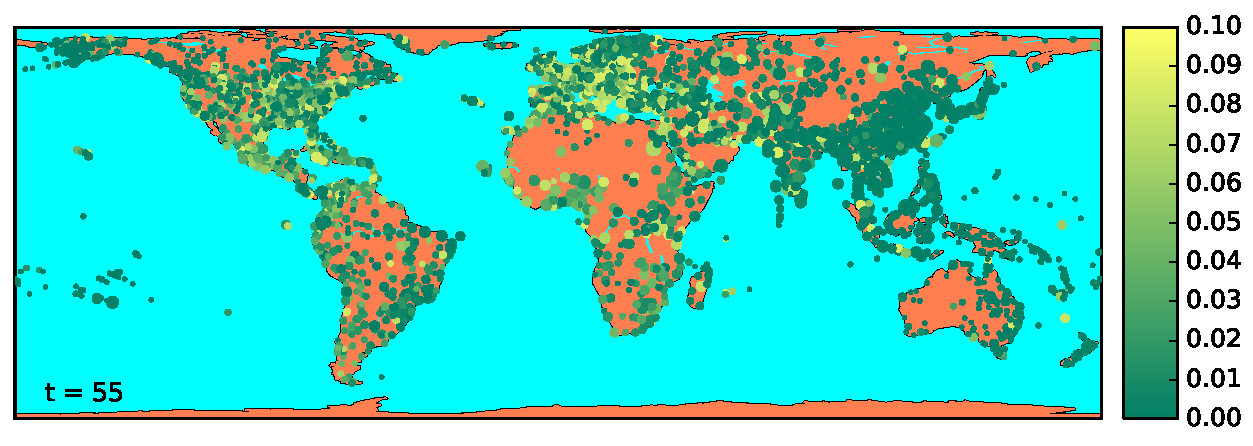
\includegraphics[width=1.0 \linewidth]{plots/gifs/frames/noRio-55}
	\caption{Frame 55 of animation without Olympic Games. The full animation can be viewed as a gif at
		\url{https://andreasmadsen.github.io/course-02443-stochastic-virus-outbreaks/}}
\end{figure}



%!TEX root = main.tex
\section{Conclusion}
This report extended the deterministic SIR-model to a multi-region stochastic SIR-model. The model was tested on a small example to validate that it accurately reflects the SIR-model. Using real population and region connection data a hypothetical virus outbreak originating in Rio de Janeiro was simulated. It

\pagebreak
\appendix
\include{appendix}

\pagebreak
\printbibliography

\end{document}
